\documentclass{article} % For LaTeX2e
\usepackage{iclr2018_conference,times}
\usepackage{amsfonts}
\usepackage{amsmath}
\usepackage{amsthm}
\usepackage{booktabs}
\usepackage{comment}
\usepackage{enumerate}
\usepackage{float}
\usepackage{hyperref}
\usepackage{import}
\usepackage[inline]{enumitem}
\usepackage{multirow}
\usepackage{soul}
\usepackage{subfigure}
\usepackage{tikz}
\usepackage{url}
\usepackage{csvsimple}
\usepackage{multicol}

\usetikzlibrary{positioning}

%%%%%%%% Customizations %%%%%%%%%%
\graphicspath{ {images/} }
% Global style for description lists
\setlist[description]{style=unboxed,leftmargin=2ex}
% Global style for all network drawings in tikz
\tikzset{
every path/.style={line width=1pt}
, every node/.style={font=\tiny}
, networknode/.style={inner sep=5.0,rounded corners,fill=black!5,font=\tiny}}

%%%%%%%%% Macros %%%%%%%%%%%%%%%%%%
\newtheorem{defn}{Definition}
\newif\ifblind
\def\goldenr{1.618}
\newcommand*\textfrac[2]{
      \frac{\text{#1}}{\text{#2}}
  }
\newcommand{\TODO}[1]{TODO:{#1}}
\newcommand{\etal}{et~al.}
\def\state{s}
\def\statet{\state_t}
\def\statetp{\state_{t-1}}
\def\statehist{\state_{1:t-1}}
\def\statetn{\state_{t+1}}
\def\obs{o}
\def\obst{\obs_t}
\def\act{a}
\def\actt{\act_t}
\def\acttp{\act_{t-1}}
\def\acttn{\act_{t+1}}
\def\Obs{\mathcal{O}}
\def\ObsFunc{C}
\def\ObsFuncFull{\ObsFunc(\statet, \actt) \rightarrow \obst}
\def\ObsFuncInv{\ObsFunc^{-1}}
\def\ObsFuncInvFull{\ObsFuncInv(\obst, \statetp, \actt) \rightarrow \statet}
\def\State{\mathcal{S}}
\def\Action{\mathcal{A}}
\def\Trans{T}
\def\TransFull{\Trans(\statet, \actt) \rightarrow \statetn}
\def\TransObs{T_c}
\def\Rew{R}
\def\rew{r}
\def\rewt{\rew_t}
\def\rewtp{\rew_{t-1}}
\def\rewtn{\rew_{t+1}}
\def\RewFull{\Rew(\statet, \actt) \rightarrow \rewtn}
\def\TransObsFull{\TransObs(\statet, \obst, \actt, \rewt; \theta_T) \rightarrow \statetn}
\def\Value{V}
\def\pit{\pi_t}
\def\piDef{\pi(\acttn|\statet, \obst, \actt, \rewt; \theta_\pi) \rightarrow \pit(\acttn ; \theta_\pi)}
\def\Valuet{\Value_t}
\def\ValueDef{\Value(\statet, \obst, \actt, \rewt; \theta_\Value) \rightarrow \Valuet(\theta_\Value)}
\def\R{\mathbb{R}}
\def\E{\mathbb{E}}
\newcommand{\fix}{\marginpar{FIX}}
\newcommand{\new}{\marginpar{NEW}}
\newcommand{\LatencyOneGtOne}{Latency $1:>1$}
\newcommand{\NavAiiiCDiDiiL}{NavA3C+D\textsubscript{1}D\textsubscript{2}L}

\newcounter{Benchmark}
\newcounter{BenchmarkB}[Benchmark]
\newcommand{\ditem}[1]{\refstepcounter{Benchmark}\item[\arabic{Benchmark}. {#1}]}
\newcommand{\dditem}[1]{\refstepcounter{BenchmarkB}\item[\arabic{Benchmark}.\alph{BenchmarkB}. {#1}]}

\title{Do deep reinforcement learning algorithms really learn to navigate?}
\title{Do deep reinforcement learning algorithms really learn to navigate?}

% Authors must not appear in the submitted version. They should be hidden
% as long as the \iclrfinalcopy macro remains commented out below.
% Non-anonymous submissions will be rejected without review.

\author{Shurjo Banerjee\footnotemark[1],%
  \, Vikas Dhiman\thanks{indicates equal contribution},%
  \, Brent Griffin,%
  \, \& Jason J. Corso\\
  The Electrical Engineering and Computer Science Deparment\\
The University of Michigan\\
Ann Arbor, MI 48109, USA \\
\texttt{\{shurjo,dhiman,griffb,jjcorso\}@umich.edu} \\
}

% The \author macro works with any number of authors. There are two commands
% used to separate the names and addresses of multiple authors: \And and \AND.
%
% Using \And between authors leaves it to \LaTeX{} to determine where to break
% the lines. Using \AND forces a linebreak at that point. So, if \LaTeX{}
% puts 3 of 4 authors names on the first line, and the last on the second
% line, try using \AND instead of \And before the third author name.

%\iclrfinalcopy % Uncomment for camera-ready version, but NOT for submission.

% Document Outline
% - Summary and marketing
% - Short tutorial on Deep reinforcement learning upto Nav-A3C
% - Describe the setup:
%    + What is the game
%       * What are the constants
%       * What are the variables that will be varied
%    + Reward design
% - How the setup is varied for various arguments
% - What are the questions that we want to answer?
% - Why do we do the experiments that we do?
% - What do the experiments tell us?
% - Summary
\begin{document}
\maketitle
\begin{abstract}
  Deep reinforcement learning (DRL) algorithms have demonstrated progress in learning to find a goal in challenging environments.
  As the title of the paper by \cite{MiPaViICLR2017} suggests, one might assume that DRL based algorithms are able to ``learn to navigate'' and are thus ready to replace classical mapping and path planning algorithms, at least in simulated environments.
  Yet, from experiments and analysis in this earlier work, it is not clear what strategies these DRL algorithms are learning to navigate the mazes and find the goal.
  In this paper, we pose and study this question: are DRL algorithms doing some form of mapping and/or path-planning?  Our experiments show that the algorithms are not memorizing the maps of mazes at the testing stage but, rather, at the training stage.
  Hence, the DRL algorithms fall short of qualifying as mapping or path-planning algorithms with any reasonable definition of mapping.
  We extend the experiments in \cite{MiPaViICLR2017} by separating the set of training and testing maps and by a more systemetic coverage of the space of experiment.
  Our experiments show that the \NavAiiiCDiDiiL{} algorithm, when trained and tested on the same maps, is able to choose the shorter paths to the goal.
  However, when tested on unseen maps the algorithms utilize a bug exploration like strategy to find the goal without doing any mapping or path planning.
\end{abstract}

\section{Introduction}
%%% Outline
% 1. Navigation is important problem
% 1.5 Traditionally addressed by mapping during exploration and path
%      planning during exploitation.
% 2. End to end learning algorithms have shown promise to take over
%      mapping and path
% 3. We do not know how these algorithms work. There has been work in computer vision that shows the learning on neural network based methods can be learning totally different kind of patterns from what we would expect.
% 4 We introduce the concept of blinding to force the learning of of long term planning. We showcase improved scores over industry standard baselines.
% 5 We showcase that blinding affords an understand of the implicit abilities of these DRL agents.

% 1. Navigation is important problem
% 1.5 Traditionally addressed by mapping during exploration and path
%      planning during exploitation.
Navigation remains a fundamental problems in mobile robotics and artificial intelligence~\cite{SmChIJRR1986,ElCOMPUTER1980}.
The problem, traditionally called SLAM (Simulataneous Localization and Mapping), is classically addressed by separating the eventual task of navigation into \textit{exploration} and \textit{exploitation}. In the exploration phase, the environment is incrementally built and represented in some sort of \emph{map} data-structure. In exploitation, this data structure is used for localization and path-planning to find an optimal path to a given destination based on desired optimality criterion. These classical methods, have been explored in depth and  there have been many advances in this classical approach \cite{XXX}, it remains a difficult challenge. \textit{Either mention some examples or cite a paper that highlights the failiures of SLAM or both!} 

%
% 2. End to end learning algorithms have shown promise to take over
%      mapping and path-planning
More recently, end-to-end navigation methods---methods that attempt to  
solve the navigation problem without breaking it down into the separate parts of localization, mapping and path-planning---have gained traction.
With the recent success of Deep Reinforcement Learning (\textbf{DRL}) \cite{MnKaSiNATURE2015,MnKaSiNATURE2015}, these end-to-end navigation methods \cite{MnBaMiICML2016,SiHuMaNATURE2016,LePaKrISER2017,MiPaViICLR2017,OhChSiICML2016} forego decisions about the details that are required in the intermediate step of map building.  

Work by Mirowski \etal{} showcased agents that learned to navigate textureless environments to find desired goal locations trained on pure monocular vision - a feat that is still quite difficult for state-of-the-art monocular SLAM systems \cite{XXX}. \textit{Talk about the memory structures used - no need for any explicit path planning, slam or all that nonsense} 
The potential for simpler yet capable methods is rich on the surface.

% 3. We do not know how these algorithms work. There has been work in computer vision that shows the learning on neural network based methods can be learning totally different kind of patterns from what we would expect.
Despite this potential and recent successes, state-of-the-art DRL based methods have been confronted with their own set of problems. In line with other Deep-Learning fallacies (\textit{too negative?}), foremost among these is the difficulty in understanding the method limitations or the kind of patterns that these algorithms are understanding. The inherent black-box nature of these methods make them hard to study. 

% 4.1 We find that it is not remembering the map it is being trained on
% 4.2 We find that no path planning is  happening only, memorizing and regeneration of the sequence of steps. However, it is not 
In this work, we attempt to pull back the lid of how these networks appear to be in fact be performing this navigation. We phrase these queries within the context of exploration and exploitation as is traditional in the SLAM world. Our contributions are three-fold:
\begin{enumerate}
\item We succesively blind state-of-the art DRL agents in a curriculum fashion to gain an understanding of whether these agents can be forced to perform long-term planning in the execution of their learned navigation strategies.
\item In a bid to more easily teach agents to perform long-term planning, we introduce BLINC. BLINC, is a conceptually simple modification applicable to all DRL methods wherein agents are incentivized to blind themselves during navigation as often as possible. Extra  incentives are provided when this blindness is contiguously performed over several frames.  We showcase how agents trained via BLINC acheive better performance then current state-of-the-art methods. 
\item We showcase BLINCs great strength in affording the ability to easily query the hidden states of the networks used by these models. We use this method to gain an understanding of each agent's explicit understanding of its surroundings at given points of time.
\end {enumerate}


%% Outline
% 1. Navigation is important problem
% 1.5 Traditionally addressed by mapping during exploration and path
%      planning during exploitation.
% 2. End to end learning algorithms have shown promise to take over
%      mapping and path
% 3. We do not know how these algorithms work. There has been work in computer vision that shows the learning on neural network based methods can be learning totally different kind of patterns from what we would expect.
% 4.1 We find that it is not remembering the map it is being trained on
% 4.2 We find that no path planning is  happening only, memorizing and regeneration of the sequence of steps. However, it is not 

% 1. Navigation is important problem
% 1.5 Traditionally addressed by mapping during exploration and path
%      planning during exploitation.
Navigation remains a fundamental problems in mobile robotics and artificial intelligence~\cite{SmChIJRR1986,ElCOMPUTER1980}.
The problem is classically addressed by separating the eventual task of navigation into exploration and exploitation. 
In exploration the environment is represented in some sort of \emph{map} data-structure. 
In exploitation, the map is used for localization and path-planning to find a path to a desired destination based on given optimality criterion. 
This classical approach, traditionally called SLAM (Simulataneous Localization and Mapping), constitutes an entire subfield of robotics whose successes include the birthing of the autonomous driving industry. 
SLAM however, possesses its own limitations. Algorithms, especially those centered in vision, lack performance invariance often failing to extend results to environments that are subtly different from the ones they were trained on. As a simple example, state-of-the-art monucular SLAM methods fail when confronted with textureless environments.

More recently, end-to-end navigation methods---methods that attempt to  
solve the navigation problem without breaking it down into separate parts of localization, mapping and path-planning---have gained traction.
%
% 2. End to end learning algorithms have shown promise to take over
%      mapping and path-planning
With the recent advances of Deep Reinforcement Learning (DRL) \cite{MnKaSiNATURE2015}, these end-to-end navigation methods \cite{MnBaMiICML2016,SiHuMaNATURE2016,LePaKrISER2017,MiPaViICLR2017,OhChSiICML2016} forego decisions about the details that are required in the intermediate step of mapping.
The potential for simpler yet capable methods is rich; for example, one can optimize to store only the minimal amount of map information that is required perform the end objective of a navigation task.
One such work, \cite{MiPaViICLR2017}, has demonstrated advances in this task of navigation creating agents that are able to explore and find goals in complicated, three-dimensional worlds without the provision of any externally-supplied map like concept or memory strcutures. 

using only the first-person monocular view in randomly generated mazes. Not only their algorithm shows evidence of localization, but they also show some of evidence of better than random path planning when the goal location is randomly chosen during evaluation time. 
:q

\begin{figure}
%\rotatebox{90}{\hspace{3em}Trained on 1 map }
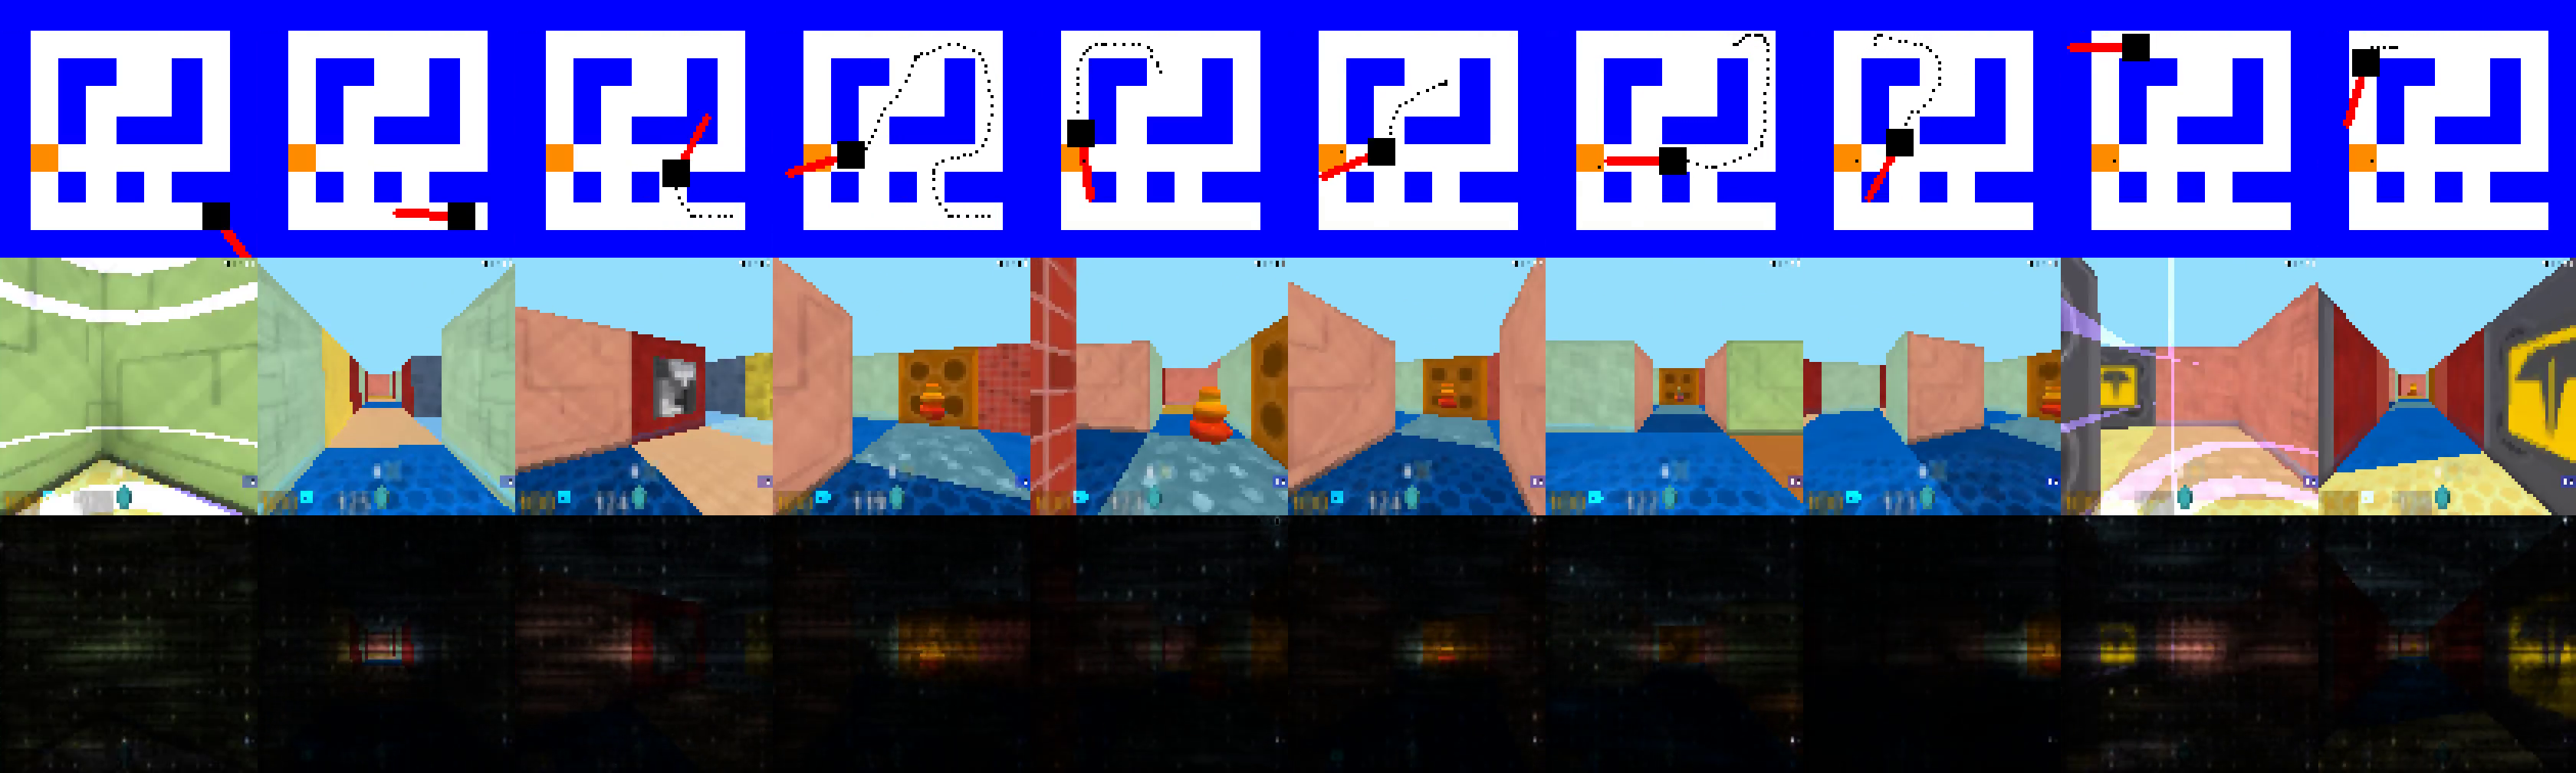
\includegraphics[width=\textwidth]{./exp-results/training-09x09-0127-on-0127.png}
%\rotatebox{90}{\hspace{2em}Trained on 1000 maps }
%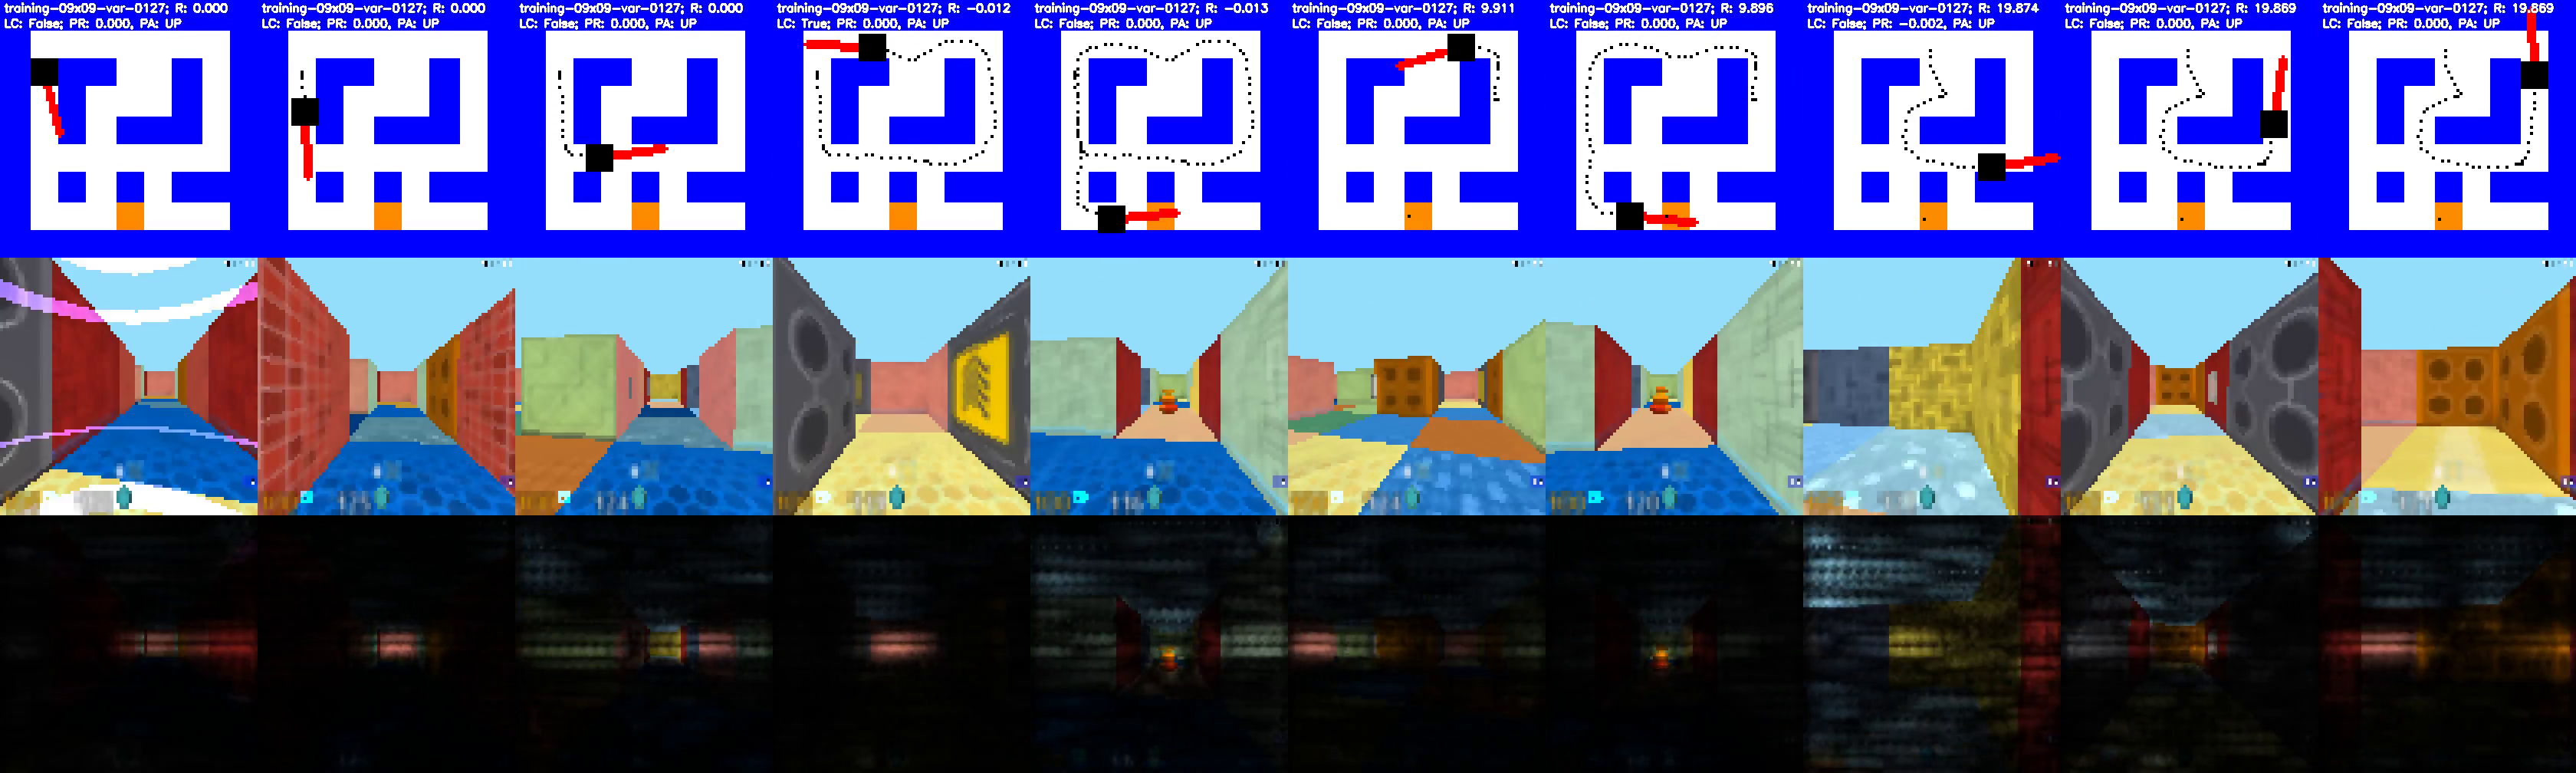
\includegraphics[width=\textwidth]{./exp-results/training-1000-on-0127.png}
\caption{Qualitative results of evaluating algorithm on map id 127. The top three rows show selected frames for the algorithm trained on the same map 127, while the bottom three rows show the result of evaluting the algorithm trained on 1000 maps evaluated on 127. The top row shows the top view of the robot moving through the maze, second row shows the first person which is the only input available to the agent (except reward). The third row shows the attention masked view of the algorithm. We observe that the algorithm focuses attention at the horizon in long corridors, on the goal object (it looks like stacked rings) and on interesting decals.}
\label{fig:training-qualitative}
\end{figure}

% 3. We do not know how these algorithms work. There has been work in computer vision that shows the learning on neural network based methods can be learning totally different kind of patterns from what we would expect.
Despite this potential and recent successes, 
state-of-the-art DRL based methods have been confronted with their own set of problems, such as difficulty to understand the method limitations or the kind of patterns the algorithm is understanding.  The black-box nature of these methods make them hard to study.
On similar lines, \cite{NgYoClCVPR2015} show that neural-network-based object detection methods can be easily fooled by introducing noise that is imperceptible to humans. Hence, it is important to analyze the DRL methods to understand if they are truly ``learning to navigate'' \cite{MiPaViICLR2017}.

% 4.1 We find that it is not remembering the map it is being trained on
% 4.2 We find that no path planning is  happening only, memorizing and regeneration of the sequence of steps. However, it is not 

In this work, we focus on the work of \cite{MiPaViICLR2017} and analyze the method using multiple random maps with different degrees of randomness. As a generalization, we propose a 4-stage benchmark for end-to-end navigation methods.
Our experimental setup is similar to \cite{MiPaViICLR2017} and uses the same open source library Deepmind's Lab \cite{BeLeTeARXIV2016}.
We setup a maze where the goal is randomly placed and the agent is randomly spawned.
The objective of the agent is to hit the goal as many times as possible within a fixed episode time.
Every time the agent hits the goal, it respawns at a random location.
With this setup \cite{MiPaViICLR2017} found that the agent finds the goal faster the second time onwards as compared to the first time.
This implies that agent is somehow able to exploit the new information about position of the goal to reach the goal faster.
However, \cite{MiPaViICLR2017} do not rule out random chance because they only show the successful result on random goal case with only one map, do not report standard deviation on their metrics and do not evaluate the algorithm on unseen maps.
Even though separting training and testing sets is the obvious thing to do in machine learning, we are the first work to evaluate any DRL based navigation method on unseen maps.
We expand on their analysis and evaluate the same metric on multiple types of maps including randomly generated maps.

We find no evidence of DRL agents being able to perform shortest path-planning in unseen mazes even in simple mazes.
We observe that the agent prefers to take a particular path just as an artifact of initialization.
We hypothesize that the agents are learning a correspondence between local sequence of frames and actions.
These findings are the results on testing and training on multiple maps that were randomly chosen from set of 1100 randomly generated maps.
We provide thorough and clear summary data to substantiate these findings as well as individual maps and results to explain them carefully.
A secondary finding is that even if the agent is trained on a single maze it is able to navigate better than random in unseen mazes.



\section{Related Work}
\paragraph{Localization and mapping}
Robotic localization and mapping for navigation is a classic problem in  mobile robotics and sensing.
\cite{SmChIJRR1986} introduced the idea of propagating spatial uncertainty for robot localization while mapping and Elfes popularized Occupancy Grids~\cite{ElCOMPUTER1980}.
In the last three decades since these seminal works, the field has exploded with hundreds of algorithms released for multiple kinds of sensors such as cameras, laser scanners, sonars and depth sensors.
Several of these algorithms have utilized varying levels of detail in the building of their map-models ranging from low-levelled ones such as topological maps \cite{KuCOGSCI1978} and sparse reconsctruction methods to high-level ones like occupancy grids and metrically accurate dense reconstructions. 

All these approaches require significant hand-tuning and design for deployment in different kinds of environments and sensor types. The level of detail utilized in the creation of the  maps also needs to be decided before hand irrespective of the application and hence the amount of information stored is not optimized for the task at hand.

\paragraph{Deep reinforcement learning}
Deep reinforcement learning (DRL) was originally conceived in 1995 \cite{TeACM1995}. 
The field gained prominence again when \cite{MnKaSiNIPSDLW2013,MnKaSiNATURE2015} used DRL to create agents that outperformed humans on Atari games while being purely trained on the games visual outputs.
Subsequently, the field has been extended in several directions \cite{MnBaMiICML2016} being applied to creation of the Alpha-GO agent\cite{SiHuMaNATURE2016}, simulated platforms \cite{KaStJoNIPS2017}, real world robots \cite{LePaKrISER2017} and more recently to robotic navigation \cite{MiPaViICLR2017,OhChSiICML2016}.

The exploration into robotic navigation using DRL is a nascent topic having the potential to disrupt the fields of simultaneous localization, mapping and path planning. However literature concerning DRL based navigation usually ignores the standard machine learning practice of separating the training and testing sets thereby limiting our understanding of the generality of these methods. In fact, it is common for agents to be trained and tested on the same maps with the variation only being applied to the agent's initial spawn point and the map's goal location \cite{MiPaViICLR2017,ZhMoKoICRA2017,KuSaGaAPA2016}. 

In contrast, \cite{OhChSiICML2016} do test on random maps but their agents are trained to choose between multiple possible goal locations based on past observations. Their episodes end when the agent collects a goal and hence there is no requirement for their methods to store map information during their exploration. Thus the decisions made by these agents are to avoid a goal of particular a color and seek other colors rather than remembering the path to the goal. On similar lines, \cite{ChLaSaNIPS2016} test their method on unseen maps in VizDoom environment but only vary the maps with unseen textures. Thus their agents are texture invariant but continue to train and test on maps with the same geometric structure.
%

In this work, we take the study of these methods significantly farther with a thorough investigation of whether DRL-based agents remember enough information to obviate mapping algorithms or whether they do in fact need to be augmented with mapping algorithms for future progress.


\section{Background}
Our problem formulation is based upon the work of \cite{MiPaViICLR2017}. We summarize the technical setup here for completeness.
We refer the reader to \cite{MnBaMiICML2016,MiPaViICLR2017} for more details of the setup.

The problem of navigation is formulated as an interaction between an environment and an agent.
At time $t$ the agent takes an action $\actt \in \Action$ and observes observation $\obst \in \Obs$ along with a reward $\rewt \in \R$.
We assume the environment to be Partially Observable Markov Decision Process (POMDP).
In a POMDP, the future state of the environment, $\statetn \in \State$, is conditionally independent of all the past states, $\statehist$, given the current state $\statet$. It is further assumed that
$\obst$ and $\rewt$ are independent of previous states given current state $\statet$ and last action $\acttp$.
Formally, a POMDP is defined as a six tuple $(\Obs, \ObsFunc, \State, \Action, \Trans, \Rew)$ that is composed of an observation space $\Obs$, an observation function $\ObsFuncFull$, a state space $\State$, an action space $\Action$, a transition function $\TransFull$ and a reward function $\RewFull$.
For our problem setup, the observation space $\Obs$ is the space of an encoded feature vector that is generated from input image along with previous action and reward.
Action space $\Action$ contains four actions: rotate left, rotate right, move forward and move backward and reward function $\Rew$ is defined for each experiment so that the reaching the goal leads to high reward with auxiliary reward to encourage certain kind of behavior.

For DRL algorithms, the state space $\State$ is not hand tuned, but it is modeled as a semantically meaningless vector of floats.
Also, instead of modeling observation function $\ObsFuncFull$ and $\TransFull$, a combined transition function $\TransObsFull$ is modeled such that it estimates the next state $\statetn$ directly considering previous observation as well as reward into account.
For policy-based DRL a policy function $\piDef$ and a value function $\ValueDef$ are also modeled.
All three functions $\TransObs$, $\pit$, $\Valuet$ share most of the parameters in a way such that $\theta_T \subseteq \theta_{\pi} \cap \theta_\Value$

%Since we aim to estimate $\ObsFuncInv$ and $\Trans$ from experience, we formulate the experience as observation tuples divided into episodes of fixed length $E$.
%Each episode experience contains $E$ tuples with observation, action and corresponding reward $D_E = \{(\obs_0, \act_0, r_0), \dots, (\obs_E, \act_E, r_E)\}$. After each episode the state $\state_t$ is reset to all zeros and another data sequence is collected. Let the collected dataset be $D_N = \{
Our objective is to estimate unknown weights $\theta = \theta_T \cup \theta_\pi \cup \theta_V$ that maximizes the expected future reward, $R_t = \sum_{k=t}^{t_{end} - t} \gamma^{k-t} r_k$, where $\gamma$ is the discount factor,
%
\begin{align}
\theta^* = \arg\max_{\theta} \E[R_t] \,.
\end{align}
%
% need \graphicspath{{images/}}
%\def\svgwidth{0.25\columnwidth}%
\begin{figure}%
%\input{images/a3c-as-pomdp.pdf_tex}%
%\def\svgwidth{0.25\columnwidth}%
%\input{images/a3c-as-nn.pdf_tex}%
\begin{center}
\usetikzlibrary{positioning}
\begin{tikzpicture}
\node[networknode,fill=green!20] at (10.5, 2.5) (lstm2) {LSTM:64};
\node[networknode,fill=green!20,left=0.6 of lstm2] (lstm) {LSTM:256};
\node[networknode,fill=orange!20,left=0.8 of lstm]  (enc2) {\parbox{8ex}{CNN:32\\4x4/2x2}};
\node[networknode,,fill=orange!20,left=0.4 of enc2]  (enc) {\parbox{8ex}{CNN:16\\8x8/4x4}};
\node[left=0.4 of enc, inputvar] (It) {$I_t$:84x84x3};
\node[above=0.1 of It,inputvar] (at) {$\acttp$};
\node[below=0.1 of It,inputvar]  (rt) {$\rewtp$};
\node [right=0.8 of lstm2,outvar] (V)  {$V$, $\pi$};
\node [shift={(-0.4,0)},above=0.4 of V,auxvar] (pi)  {$L$};
\node [shift={(-0.4,0)},below=0.4 of V,auxvar] (D)  {$D_2$};
\draw [-stealth] (It) edge (enc);
\draw [-stealth] (at) edge [in=110,looseness=0.4] (lstm2);
\draw [-stealth] (enc2) edge [bend left=70,looseness=0.4] (lstm2);
\draw [-stealth] (enc) edge (enc2);
\draw [-stealth] (enc2) edge node [shift={(0.225,0.1)},left]{$o_t$} (lstm);
\draw [-stealth] (rt) edge  [bend right,looseness=0.3] (lstm);
\draw [-stealth] (lstm) edge node[below=0.4,auxvar] (D1) {$D_1$} (lstm2);
\draw [-stealth] (lstm) edge [bend left] (D1);
\draw [-stealth] (lstm2) edge [bend right] (pi);
\draw [-stealth] (lstm2) edge  (V);
\draw [-stealth] (lstm2) edge [bend left] (D);
%\draw [use as bounding box] (5.0,1.5) rectangle (12.0, 4.0);
\end{tikzpicture}
%
\end{center}
%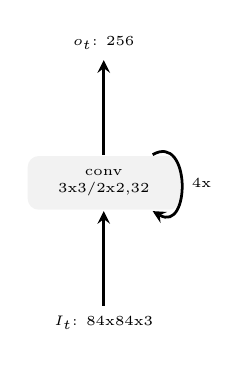
\begin{tikzpicture}
%\draw [use as bounding box] (0,0) rectangle (1.8in, 3in);
\node[] at (2.3, 2) (It) {$I_t$: 84x84x3};
\node[networknode, above=1.2 of It, text width=45, align=center] (c1) {conv\\
  3x3/2x2,32};
\node[above=1.2 of c1] (ft) {$o_t$: 256};
\draw [-stealth] (c1) edge [out=30, in=-30,looseness=2] node [right] {4x}(c1);
\draw [-stealth] (It) -- (c1);
\draw [-stealth] (c1) -- (ft);
\end{tikzpicture}
\hspace{-1ex}%
%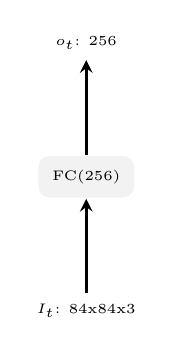
\begin{tikzpicture}
%\draw [use as bounding box] (0,0) rectangle (1.8in, 3in);
\node[] at (2.3, 2) (It) {$I_t$: 84x84x3};
\node[networknode, above=1.2 of It] (fc) {FC(256)};
\node[above=1.2 of fc] (ft) {$o_t$: 256};
\draw [-stealth] (It) -- (fc);
\draw [-stealth] (fc) -- (ft);
\end{tikzpicture}
%
\caption{Modified \NavAiiiCDiDiiL{} (\cite{MiPaViICLR2017}) architecture.
The architecture is has three inputs the current image $I_t$ and previous action $\acttp$ and previous reward $\rewtp$.
As shown by \cite{MiPaViICLR2017}, the architecture improves upon vanilla A3C architecture by using auxiliary outputs of loop closure signal $L$ and predicted depth $D_1$ and $D_2$.
Since we use a smaller action space then \cite{MiPaViICLR2017} and our agent moves with constant velocity, we do not use velocity at previous time step as input signal.}
\label{fig:architectures}
\end{figure}

\paragraph{Asynchronous Advantage Actor-Critic}
\def\charelig{\nabla_{\theta_\pi}\ln \pit(\acttn; \theta_\pi)}
% There are many different variations of RL. There are many different RL algorithms: value-based methods like Q-learning and SARSA and policy-based method like actor-critic.
In this paper we use the policy-based method called Asynchronous Advantage Actor-Critic (A3C) (\cite{MnBaMiICML2016}) that allows weight updates to happen asynchronously in a multi-threaded environment.
It works by keeping a ``shared and slowly changing copy of target network'' that is updated every few iterations by accumulated gradients in each of the threads.
The gradients are never applied to the local copy of the weights, but the local copy of weights is periodically synced from the shared copy of target weights.
The gradient for the weight update is proportional to the product of \emph{advantage}, $R_t - \Value_t(\theta_\Value)$, and \emph{characteristic eligibility}, $\charelig$ (\cite{WiML1992}), updating the weights according to the following update equations
\begin{align}
  \theta_\pi &\leftarrow \theta_\pi
  + \sum_{t \in \text{episode}}\alpha_\pi \charelig (R_t - \Value_t(\theta_\Value))
  \\
  \theta_\Value &\leftarrow \theta_\Value
  + \sum_{t \in \text{episode}} \alpha_\Value \frac{\partial (R_t - \Value_t(\theta_\Value))^2}
                  {\partial\theta_\Value}
                  \, .
\end{align}

For more details of the A3C algorithm we refer the reader to \cite{MnBaMiICML2016}.
\paragraph{\NavAiiiCDiDiiL{}}
In this work we use the \NavAiiiCDiDiiL{} architecture as proposed by \cite{MiPaViICLR2017} which builds modifying the network architecture to have two LSTMs and with auxiliary outputs of depth predictions along with loop closure predictions.
The schematic of the architecture is shown in Fig~\ref{fig:architectures}.
The architecture is has three inputs the current image $I_t$ and previous action $\acttp$ and previous reward $\rewtp$.
As shown by \cite{MiPaViICLR2017}, the architecture improves upon vanilla A3C architecture by using auxiliary outputs of loop closure signal $L$ and predicted depth $D_1$ and $D_2$.
Since we use a smaller action space then \cite{MiPaViICLR2017} and our agent moves with constant velocity, we do not use velocity at previous time step as input signal.



\section{The DRL Navigation Challenge}
%VD: a subheading immediately after a headng should be avoided
%\subsection{Setup}
Since deep reinforcement learning algorithms need millions of iterations to train, in the absence of thousands of robotic replicas like \cite{LePaKrISER2017}, we evaluate the algorithms on a simulated environment.
We use the same game engine as \cite{MiPaViICLR2017}, called Deepmind Lab (\cite{BeLeTeARXIV2016}).
The game is setup such that an agent is placed within a randomly generated maze containing a \emph{goal} at a particular location.
On reaching the goal, the agent \emph{re-spawns} within the same maze while the goal location remains unchanged. 
Following \cite{MiPaViICLR2017}, we scatter the maze with randomly placed smaller apple rewards (+1) to encourage initial explorations and assign the goal a reward of +10.
% VD: Defining the objective in terms of reward is wrong because designing rewards is a part of reinforcement learning not the problem statement.
The agent is tasked to find the goal as many times as possible within a fixed amount of time, re-spawning within the maze, either statically or randomly, each time it reaches the goal.
% JJC: TODO: remind that the spawn location can be random or static

Unlike \cite{MiPaViICLR2017}, we include a small wall penalty (-0.2) that pushes the agent away from the wall.
% VD: Do we need experiments to support that?
% VD: It is not clear how wall penality will avoid backward motion. Let's avoid that argument.
The wall penalty is useful to prevent agents from moving along the walls, thereby discarding vision input for exploration.
% Reward formulation
%The setup of game is such that it enables evaluating the algorithm for optimal path planning as well as enable dividing experiments into exploration and exploitation stages.
%We introduce a metric that evaluates how well the agent exploits the information gained during exploration before finding the goal for the first time.
% The optimal way of finding the goal in fastest way is to collect
% enough information for creating a map and use the map to find the shortest path from start to end location.
% However, an end-to-end navigation algorithm might find other ways of finding optimal strategies to find the goal.
We also use a discrete 4-action space (move forward/backward, rotate left/right)which is different from the 8-action space one used by \cite{MiPaViICLR2017}.
% VD: Do we need to show experiments for these claims?
% JJC: TODO: explain why this won't effect the comparability of results.
A smaller action space helps the algorithm train faster while achieving similar reward values.
% VD: this will raise more questions like why grounding in vision is necesary
% The agent's picking up of rewards is thus explicitly grounded in its vision as the agent must rotate in the direction of motion during exploration.

We generate 1100 random maps using depth-first search based maze generation methods.
More information on maze generation can be found in the appendix. 
Of the first 1000 maps, 10 are randomly selected for our static-map experiments (Fig. \ref{fig:environments}). For our unseen map experiments, agents are trained on increasing subsets of the first 1000 maps and tested on the remaining 100.
Unlike \cite{MiPaViICLR2017} and similar to \cite{ChLaSaNIPS2016}, we use randomly textured walls in our mazes so that the policies learned are texture-independent.

\paragraph{Evaluation Metrics}
We evaluate the performance in terms of three metrics: rewards, \emph{distance traveled : shortest path} and \emph{\LatencyOneGtOne{}}.
The metric \emph{distance traveled : shortest path} is defined as the ratio of total distance traveled by the agent versus the sum of approximate shortest distances to the goal.
The shortest distance between the spawn point and goal location is computed in the block world and hence is only an approximation of the shortest distance. 
Following \cite{MiPaViICLR2017}, we report \emph{\LatencyOneGtOne{}}, a ratio of the time taken to hit the goal for the first time (exploration time) verses the average amount of time taken to hit goal subsequently (exploitation time).
The metric is a measure of how efficiently the agent exploits map information to find a shorter path once the goal location is known. 
If this ratio is greater than 1, the agent is doing better than random exploration and the higher the value, the better its map-exploitation ability.

% VD: Let's describe this terminology in the descriptions of tasks
% Througout our experiments we refer to goal locations, spawn locations and maps as static or random.
% When static is used for spawn and goal location, they described positions that remain fixed through all episodes during both the training and the testing.
% When random is used, the spawn location changes randomly throughout the duration of the episode for both training and testing. When used for the goal, random means that its locations changes between episodes for training and testing. During the course of an episode, however, a random goal remains in the same position allowing for agents that exploit map information to find it repeatedly and thus maximize reward.
% In the context of maps, statics maps imply that the same map is used for training and testing. Random means that agents are simulataneously trained on multiple maps and tested on previously unseen ones.

\subsection{Experiments}
\label{sec:navtasks}
We evaluate the Nav-A3C algorithm on maps with 5 stages of difficulty. While the Nav-A3C algorithm works smoothly on the easier stages, it does not perform better than bug-exploration methods on the hardest stage.
We propose these experiments as a 5-stage benchmark for all end-to-end navigation algorithms.

%While there already exists optimal algorithms to find shortest path between two points and perform optimal navigation between given set of points in a given map, the advantage of Deep reinforcement learning comes from its ability to extract required features from the input images and its promise
%optimize mapping and path planning in end-to-end fashion. 
%Thus we need to either integrate existing path planning and mapping methods with deep learning methods to perform end-to-end training or extend deep learning methods to learn path planning and mapping.

\begin{description}
  \ditem{Static goal, static spawn, and static map}
  \label{prob:sss}
  % VD: Ask people if the name of the experiment makes it clear
  %In this setup, we keep the goal location, spawn location and the map fixed during both training and testing.
  %This is the easiest variation of our experiments with the environment being deterministic. 
  To perform optimally on this experiment, the agent needs to find and learn the shortest path at training time and repeat it during testing. 

  \ditem{Static goal, random spawn and static map}
  % VD: Probably clear from the name
  % In this setup, we keep the goal location and the map fixed during both training and testing but chose a random spawn point every time the agents re-spawns.
  This is a textbook version of the reinforcement learning problem, especially in gridworld \cite{SuBaBOOK1998}, with the only difference being that the environment is partially observable instead of fully observable.
  This problem is more difficult than Problem~\ref{prob:sss} because the agent
  must find an optimal policy to the goal from each possible starting point in the maze.
  \ditem{Random goal, static spawn, and static map}
  % VD: The randomness of the goal is what we need to qualify
  In this setup, we keep the spawn location and the map fixed during both training and testing but chose a random goal location for each episode.
  Note that the goal location stays constant throughout an episode.
  % VD: This line does not add any information
  %This experiments highlights the map-exploitation ability of the agent.
  The agent can perform well on this experiment, by remembering the goal location after it has been discovered and exploiting the information to revisit goal faster.  
  
  Following \cite{MiPaViICLR2017}, we report the ratio
  of time taken to hit the goal for the first time (exploration time) vs the average amount of time taken to hit goal subsequently (exploitation time). The metric, called \emph{\LatencyOneGtOne{}}, is a measure of how efficiently the agent exploits map information to find shorter path once the goal location is known. 
  If this ratio is greater than 1, then we say that the agent is doing better than random exploration and higher values is better.
  \ditem{Random goal, random spawn, and static map}
  In this version of the experiment both the spawn point and the goal location is randomized. To perform optimally, the agent must localize itself within the map in addition to being able to exploit map-information.
  
  This is the problem that is addressed by \cite{MiPaViICLR2017} with limited success. 
  They evaluate this case on two maps and report \LatencyOneGtOne{} to be greater than 1 in one of the two maps. We evaluate the same metric on ten other maps and provide the tools for application to several more.
  \ditem{Random goal, random spawn, and random map}
    We believe that any proposed algorithms on end-to-end navigation problems, should be evaluated on unseen maps.
    To our knowledge, this is the first paper to do so in the case of deep reinforcement learning based navigation methods.
    We train agents to simultaneously learn to explore 1, 10, 100, 500 and 1000 maps and test them on the same 100 unseen maps. The relevant results can be found in Fig~\ref{fig:num-training-maps} and discussed in Section~\ref{sec:analysis}.
\end{description}

The comparative evaluation of the different the stages of this benchmark are shown in Fig~\ref{fig:latency-goal-reward} and expanded upon in the next section.

%\subsection{Evaluation Maps}
%We evaluate our trained models on a few qualitative maps previously unseen during training time. Each of these maps have two paths to the goal. 
%We evaluate the percentage of times the agent travels to the goal along the shortest path after discovering it in the exploitation phase. 
%The purpose of these maps is to quantitavely evaluate whether these trained models can translate map-exploitative abilities to new, unseen maps. 
%
%\setcounter{Benchmark}{0}
%\begin{description}
%    \ditem{Square Map}
%        
%    \ditem{Wrench map}
%    This map is shown on the top row, extreme right column in Fig~\ref{fig:environments}. It has one loop and a corridor.
%    The goal is placed asymmetrically in the loop and the agent is spawned in the corridor.
%    Because of asymmetrical placement of the goal, one of the path to the goal is shorter than the other and there are only two possible paths.
%    We record the path taken each time. If the agent has learned a greedy strategy, then it would repeat the path taken for the first time.
%    We evaluate the fraction of times, the agent repeats the first path. A higher number indicates a greedy strategy.
%    In second evaluation, we let the agent explore randomly untill it hits the goal via the shorterst path.
%    At this point we evaluate the  fraction of times shortest path is taken. For this score 
%    \ditem{Goal map}
%    This map is shown on the bottom row, extreme right column in Fig~\ref{fig:environments}.
%    We chose this map because this is the simplest map with a fork. Making the map any simpler will make the map homeomorphic to a straight line. 
%    We evaluate the number of times the agent takes the right descision at the fork after exploring the goal once.
%\end{description}

% \begin{figure}%
% 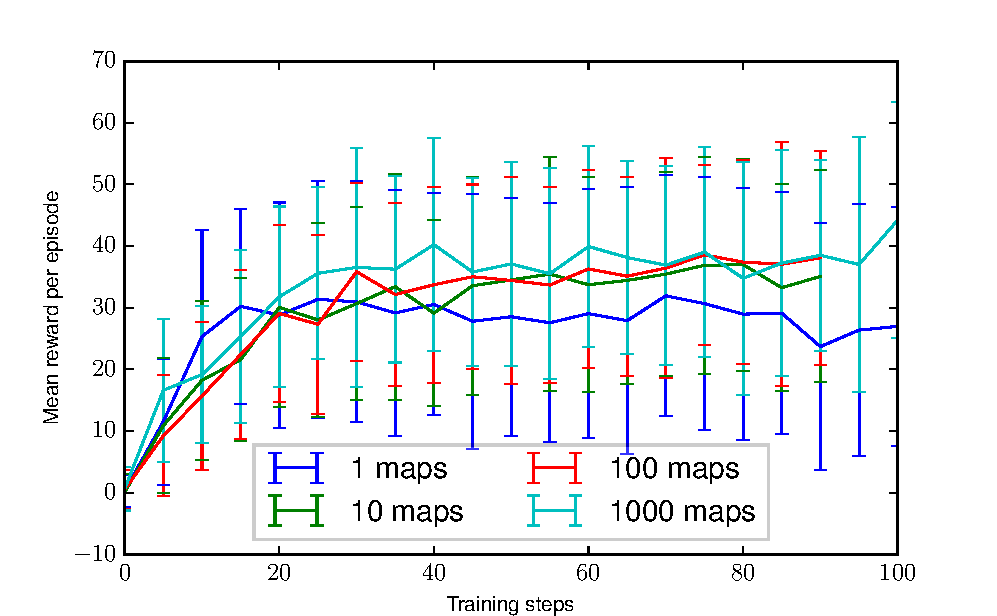
\includegraphics[width=0.5\columnwidth]{images/plot_reward_3D-1000.pdf}%
% 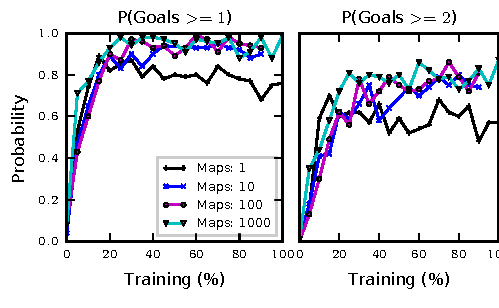
\includegraphics[width=0.5\columnwidth]{images/plot_probability_3D-1000.pdf}%
% \vspace{-1em}%
% \caption{Mean reward while tested on 100 unseen maps, while being trained on different number of training maps. Note that while training on 1000 maps eventually achieves high reward, it is only higher mean reward (44.2), training on 1 map hits the maximum (31) much faster.}%
% \label{fig:plot_reward_on_testing}%
% \end{figure}


%We evaluate the Nav-A3C\cite{MiPaViICLR2017} algorithm on randomly chosen ten maps with increasing difficulty.
%The results of our experiments are shown in Fig~\ref{fig:latency-goal-reward}.
%We change the randomness of either the spawn point or the goal location.
%We note that the increasing randomness gradually reduce the maximum reward achived and the number of times the goal is reached. As expected, the variance in reward and number of times goals is reached also increases with randomless.
%

%\subsection{Evaluation Metrics}
%We report three evaluation metrics in all our experiments: reward, average number of goal hits and \LatencyOneGtOne{}. We run evaluations on a map for 100 episodes and take the mean and standard deviation of the rewards per episode and number of goal hits per episode. Even though reward includes rewards due to apples and negative rewards due to wall penalities, the reward due to goal dominates dominates the reward metric making reward approximately ten times the average goal hits.
%
%The \LatencyOneGtOne{} is defined as the ratio of time take to find the goal first time to the average time take to find goal thereafter.
%Note that whenever the goal location is ``Random'' (different in each episode but same for the episode), untill the goal is found for the first time, the agent is just exploring the map.
%After the first goal hit, the agent should be able to exploit the location of the goal to find the goal in shorter times.
%Hence a \LatencyOneGtOne{} value greater than one indicates that the algorithm is able to successfully exploit information gathered during goal finding exploration.
%


\section{Results and Analysis}
\label{sec:analysis}
\begin{figure}%
  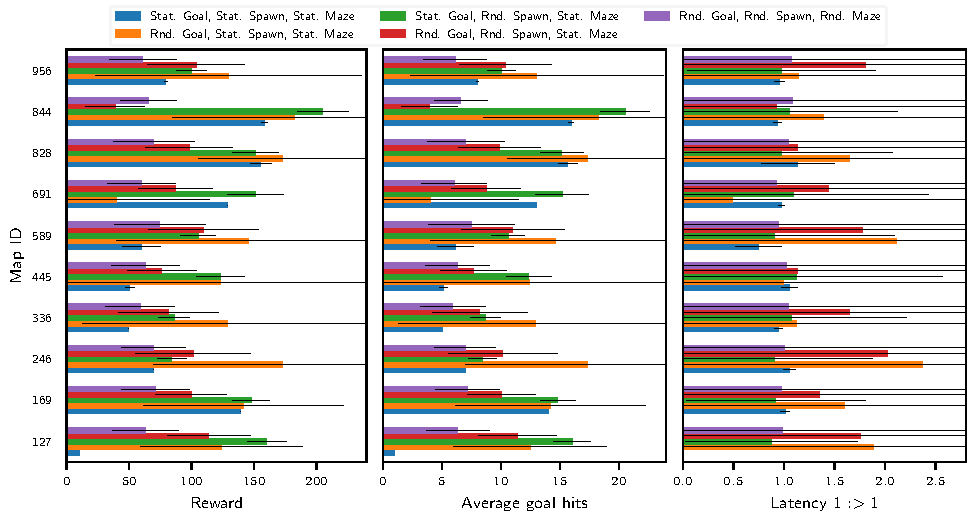
\includegraphics[width=\linewidth]{images/plot_summary_bar_plots.pdf}%
  \vspace{-1em}%
  \caption{
    We evaluate the \NavAiiiCDiDiiL{}~\cite{MiPaViICLR2017} algorithm on ten randomly chosen maps with increasing difficulty as described in Sec~\ref{sec:navtasks}.
  Vertical axis is one of the ten maps on which the agent was trained and evaluated.
  Horizontal axes are different evaluation metrics.
  We note that when the goal is static then rewards are consistently higher as compared to random goal while static spawn location and random spawn location are roughly close to each other within bounds of uncertainity. As expected, switching each variable from static to random increases the standard deviation on the results.
  From the \LatencyOneGtOne{} results we note that the current state of art algorithms do well when trained and tested on the same map but fail to generalize to new maps when evaluated on ability to exploit the information about goal location.
  Also note that \LatencyOneGtOne{} metric for cases of static goals is expected to be close to one because the location of goal is learned at train time.
  }%
\label{fig:latency-goal-reward}%
\end{figure}

\begin{figure}[t!]%
\centering%
\def\figw{0.16\columnwidth}%
\newcommand{\includesnapshot}[1]{%
  \includegraphics[width=\figw,trim=336pt 0 0 0,clip]{#1}}%
\includesnapshot{images/snapshot/00063000-snapshot.png}%
\includesnapshot{images/snapshot/00087000-snapshot.png}%
\includesnapshot{images/snapshot/00156165-snapshot.png}%
\includesnapshot{images/snapshot/00159840-snapshot.png}%
\includesnapshot{images/snapshot/00166605-snapshot.png}%
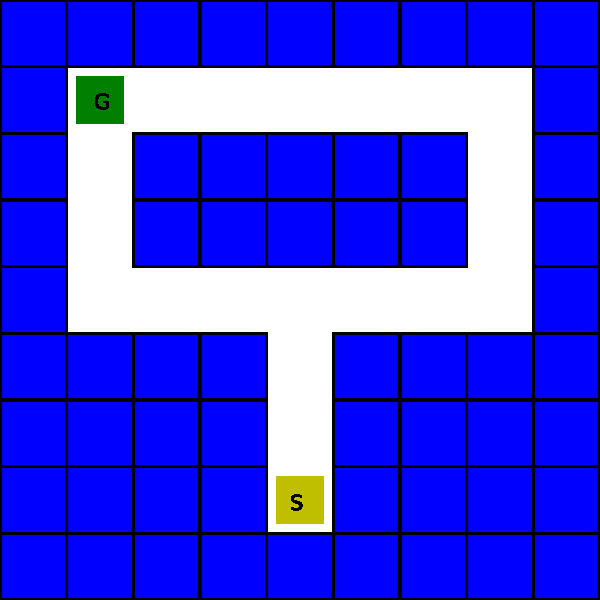
\includegraphics[width=\figw]{images/dhiman_0002_entityLayer.pdf}\\
\includesnapshot{images/snapshot/00193065-snapshot.png}%
\includesnapshot{images/snapshot/00338220-snapshot.png}%
\includesnapshot{images/snapshot/00344985-snapshot.png}%
\includesnapshot{images/snapshot/00948930-snapshot.png}%
\includesnapshot{images/snapshot/00956325-snapshot.png}%
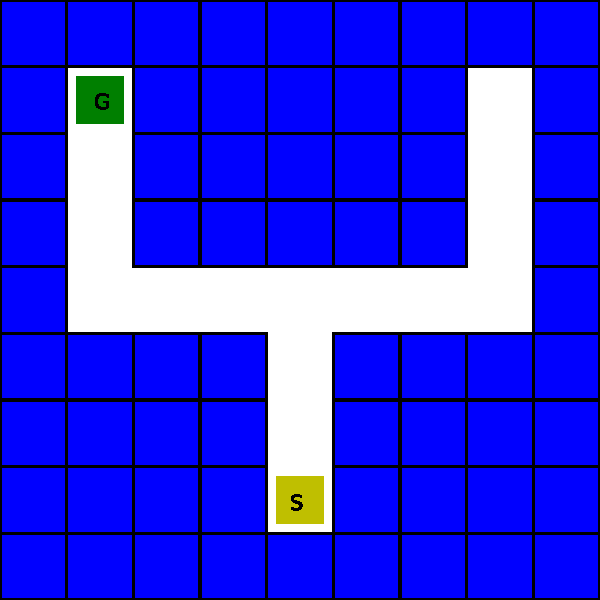
\includegraphics[width=\figw]{images/dhiman_0003_entityLayer.pdf}\\
\caption{A mazes sampled from the randomly generated mazes}%
\label{fig:environments}
\end{figure}


The results for the DRL Navigation challenge are shown in Fig~\ref{fig:latency-goal-reward} and described below.

\subsection{Metric Evaluations}
\paragraph{static goal, static spawn, static maze} In this simplest case, the agents memorizes the a path to the goal during training and repeats it during testing. The reward is high, and both the \LatencyOneGtOne{} and distance-efficiency is close to 1 with small standard deviations implying the path chosen is the shortest available.

\paragraph{Static goal, random spawn, static map}

We note that when the goal is static the rewards are consistently higher as compared to when it is random. In the case of static versus random spawn locations, rewards are close to each other within bounds of uncertainty. As expected, switching each variable from static to random increases the standard deviation on the results.
  From the \LatencyOneGtOne{} results we note that the current state of art algorithms do well when trained and tested on the same map but fail to generalize to new maps when evaluated on ability to exploit the information about goal location.
  Also note that \LatencyOneGtOne{} metric for cases of static goals is expected to be close to one because the location of goal is learned at train time.

\subsection{Evaluation on unseen maps}
The results for training on $N$ maps, where $N \in \{10, 100, 500, 1000\}$, and testing on 100 unseen maps are shown in Fig~\ref{fig:num-training-maps}.
We observe that there is a significant jump of average reward and average goal hits when the number of training maps is increased from 10 to 100 but no significant increase when the number of training maps are increased from 100 to 500 to 1000.
This is due to the fact that the wall-following strategy learned by the algorithm,
is learned with enough variation in 100 maps and training on additional maps does not add to the learned strategy.

\subsection{Effect of apples and texture}
We evaluate the effect of apples and texture during evaluation time in Fig~\ref{fig:num-training-maps}.
We train the algorithm on randomly chosen training maps with random texture and evaluate them no maps with and without random texture and also on maps with and without apples. When the apples are present, we place the apples with probability 0.25 in each block of the map.
We find that the algorithm, being trained on random textures and random placement of apples, is robust to presence or absence of textures and apples.


\subsection{Qualitative evaluation on simple maps}
% 1. We test the trained algorithms on simple maps.
To evaluate what strategies that the algorithm is employing to reach the
goal we evaluate the algorithm on very simple maps where there are only two
paths to reach the goal. The qualitative results for the evaluation are shown
in Fig~\ref{fig:planning-qualitative}.

\begin{figure}%
  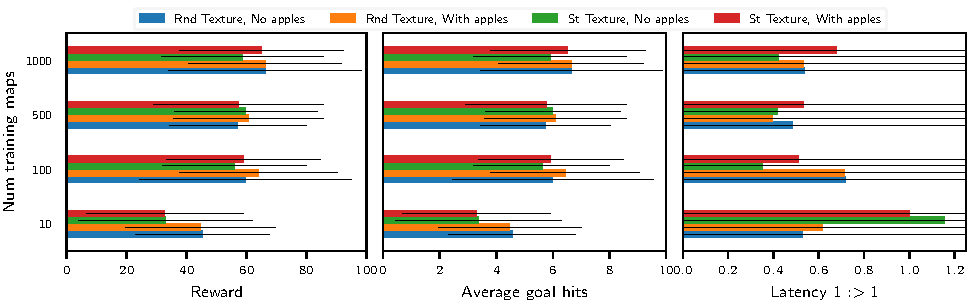
\includegraphics[width=\linewidth]{images/plot_ntrain_summary.pdf}%
  \caption{Plots showing the effect of number of training maps with random texture (Rnd Texture) and presence of apples (With apples), when evaluated on unseen maps. We note that although the difference between mean metrics is negligible as compared to standard deviation of the metrics. Hence we say that the effect of apples or textures can be ignored.
  The only clear trend is apparent \LatencyOneGtOne{} metric which suggest that random texture along without apples is advantageous in exploiting goal location while finding the goal second time on-wards.}
  \label{fig:num-training-maps}
\end{figure}

\paragraph{Square map}
% 3. In the square map, we find that the path taken is in the
%    direction of pose initialization. the visualization of path taken is
%    shown in Fig. . the correlation with of path taken with initial pose
%    is shown in Fig. . The correlation with shortest path is shown in
%    Fig. . Hence, the algorithm instead of shortest path planning takes the
%    the direction in which it is initialized.
A Square map (Fig~\ref{fig:planning-qualitative}) is the simplest possible map with two paths to the goal.
We evaluate the algorithm trained on 1000 random maps on square map.
We observe that the agent greedily moves in the direction of
initialization.
This may be because of the initial learning which is
motivated by small rewards of getting apples.
We compute the percentage of times the agent takes the shortest path over a trial of 100 episodes.
We find the agent takes the shortest path only $50.4$\% ($\pm 12.8$\%) of the times, no better than random.
% Quantitative result taken from:
% exp-results/planning-09x09-0002/gen_stats_latest_loaded-from-training-1000_acting-on-planning-09x09-0002_vars-True_apples-0.json

\paragraph{Wrench map}
% 2.2 To eliminate the correlation with initial orientation, we start
%     with wrench map. The spawn point is guaranteed to be initialized in
%     the handle of the wrench. Hence, the decision point is the only
%     junction in the map where the algorithm either decides to take a
%     left or a right.
%     We find no correlation between shortest path and the direction taken. 
To eliminate the dependency on initial orientation, we evaluate the algorithm on Wrench map as shown in Fig~\ref{fig:planning-qualitative}. We fix in the spawn point at the bottom of the tail so that shortest path is independent of the spawn orientation.
The decision about the shortest path is made at the junction where the agent can either chose to go left or right.
We find that the agent is taking shortest path only $32.9$\% ($\pm 25.1$\%) of the times which is again to better than random.
% Quantitative result taken from:
% exp-results/planning-09x09-0004/gen_stats_latest_loaded-from-training-1000_acting-on-planning-09x09-0004_vars-True_apples-0.json

% Goal map provides a similar independence from starting orientation
% but the penalty for choosing the wrong path is much higher than the
% wrench map. 
\paragraph{Goal map}
Similarly to the wrench map, the goal map (Fig~\ref{fig:planning-qualitative}) provides a decision point independent of the initial orientation, but it penalizes the wrong decision more than the wrench map $42.6$\% ($\pm 35.1$\%) of the times which is again no better than random.
% Quantitative result taken from:
% exp-results/planning-09x09-0006/gen_stats_latest_loaded-from-training-1000_acting-on-planning-09x09-0006_vars-True_apples-0.json

% JJC: TODO: Summarize results on simple maps
These experiments show that \NavAiiiCDiDiiL{} algorithm, even when trained on 1000 maps, do not generalize to these very simple maps.
Again note that even in cases when there are only two possible paths to the goal, the agent is unable to chose the shorter path with more than 50\% probability.
This shows that the models trained on 1000 maps have learned only a wall-following strategy rather than learning to plan path based on goal location.

%\subsubsection{Qualitative results}
\begin{figure}[h]
\def\vertspace{1ex}
\rotatebox{90}{\hspace{1ex}\tiny Square map}%
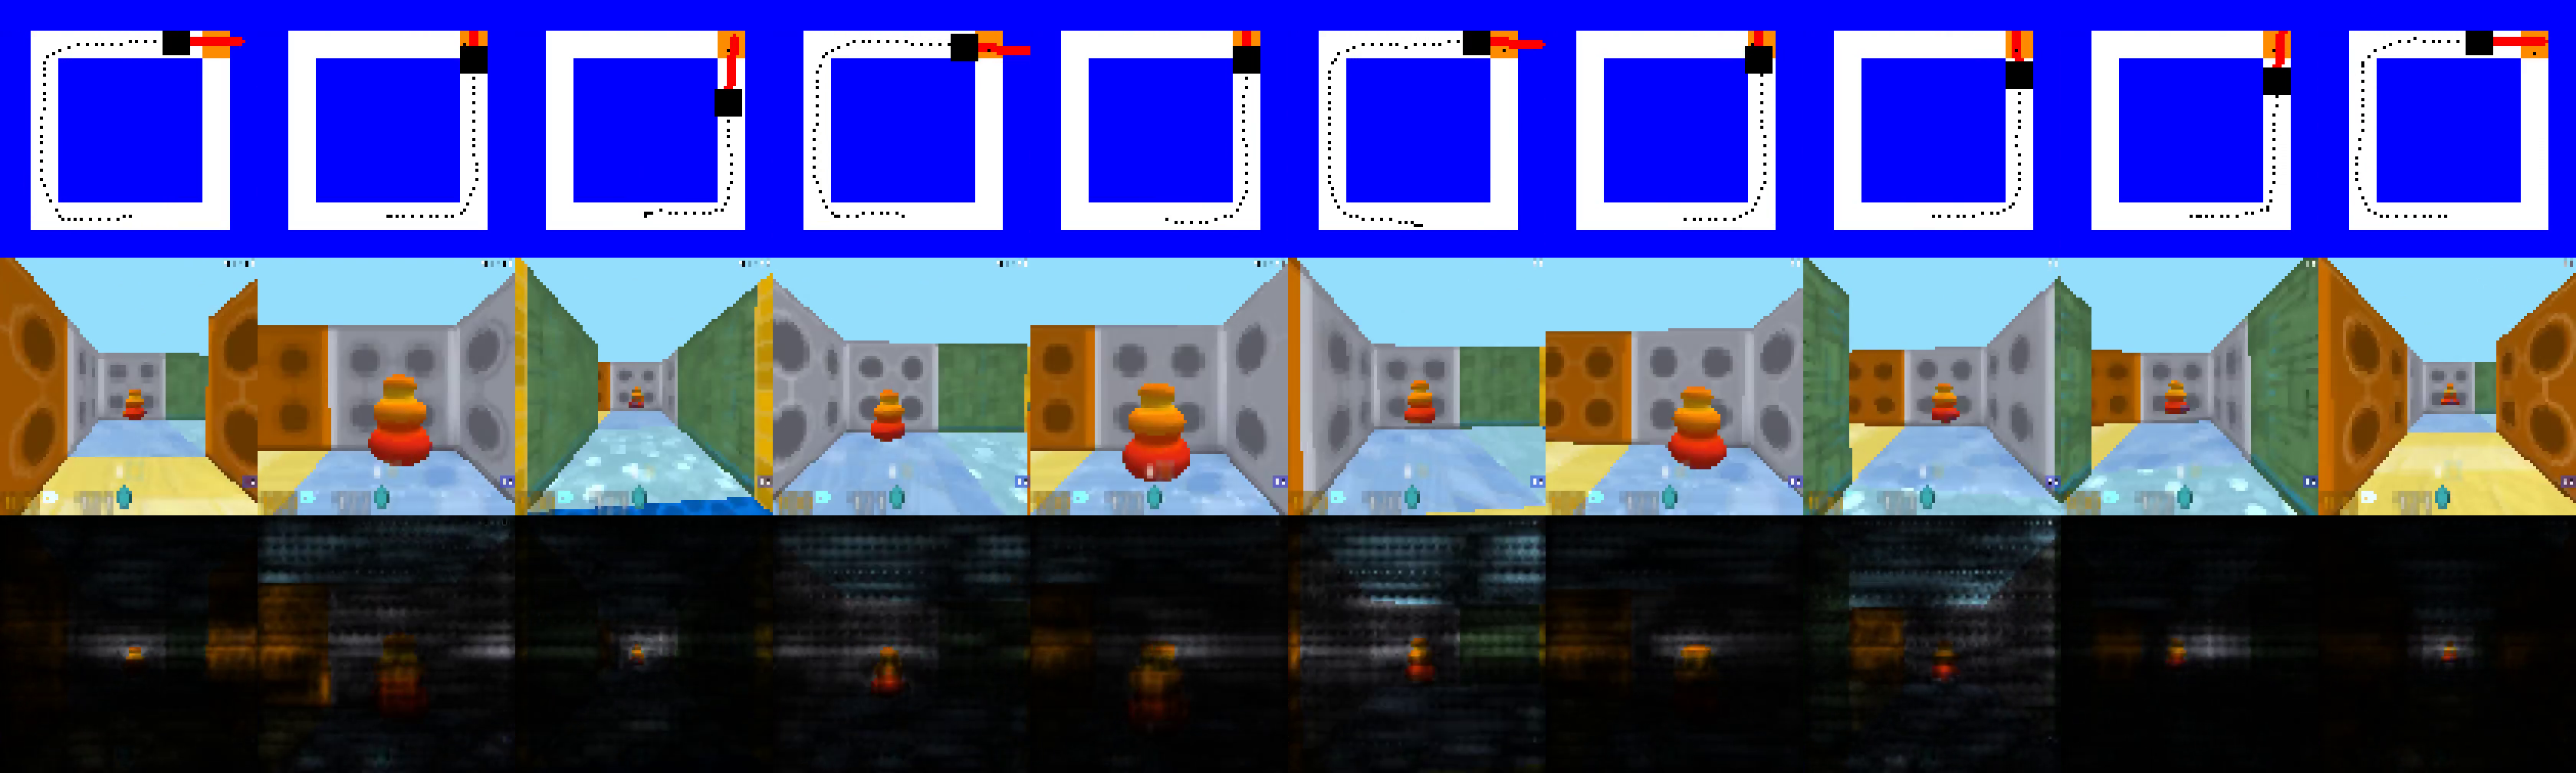
\includegraphics[width=0.98\textwidth,trim=0 672pt 0 0,clip]{./exp-results/training-1000_on_square_map.png}%
\vspace{\vertspace}
\rotatebox{90}{\hspace{1ex}\tiny Wrench map}%
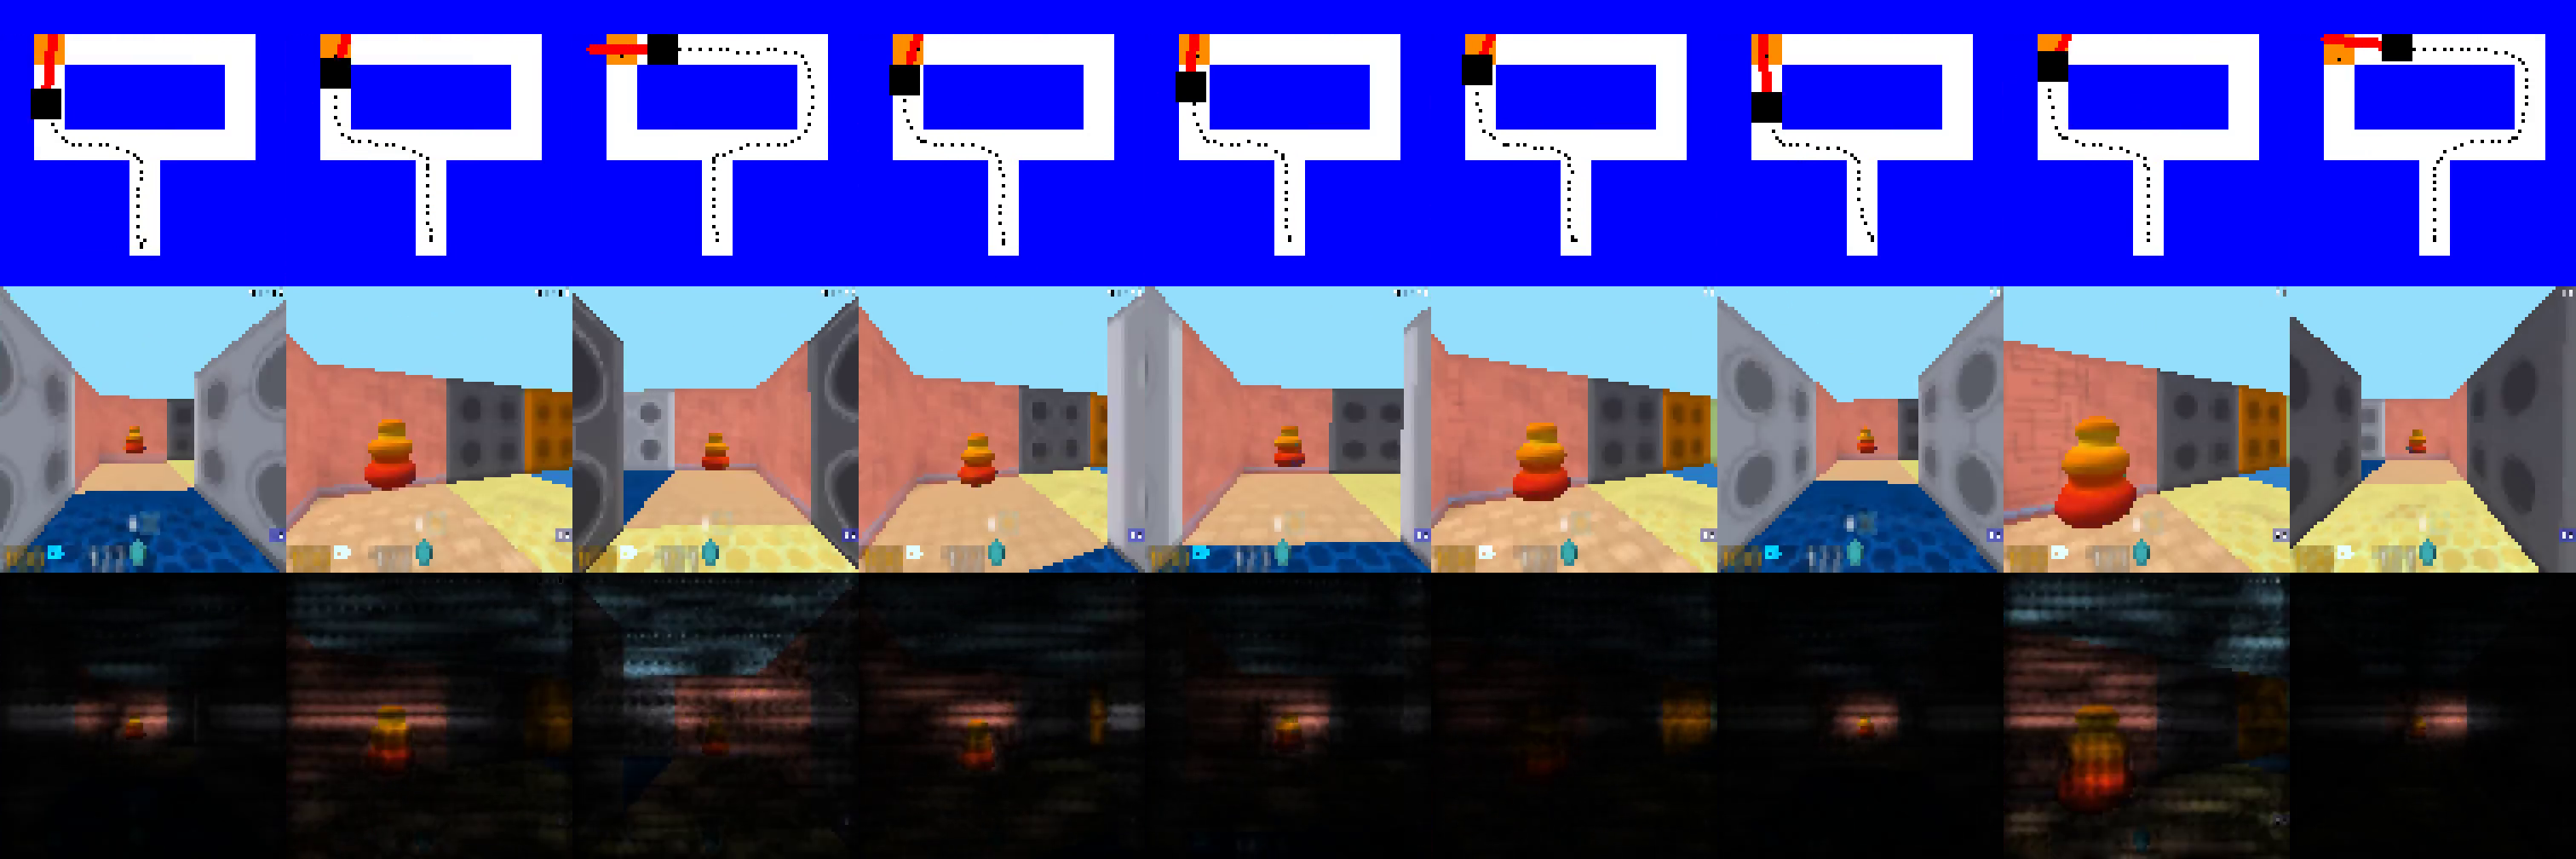
\includegraphics[width=0.98\textwidth,trim=0 672pt 0 0,clip]{./exp-results/training-1000_on_wrench_map.png}%
\vspace{\vertspace}
\rotatebox{90}{\hspace{2ex}\tiny Goal map}%
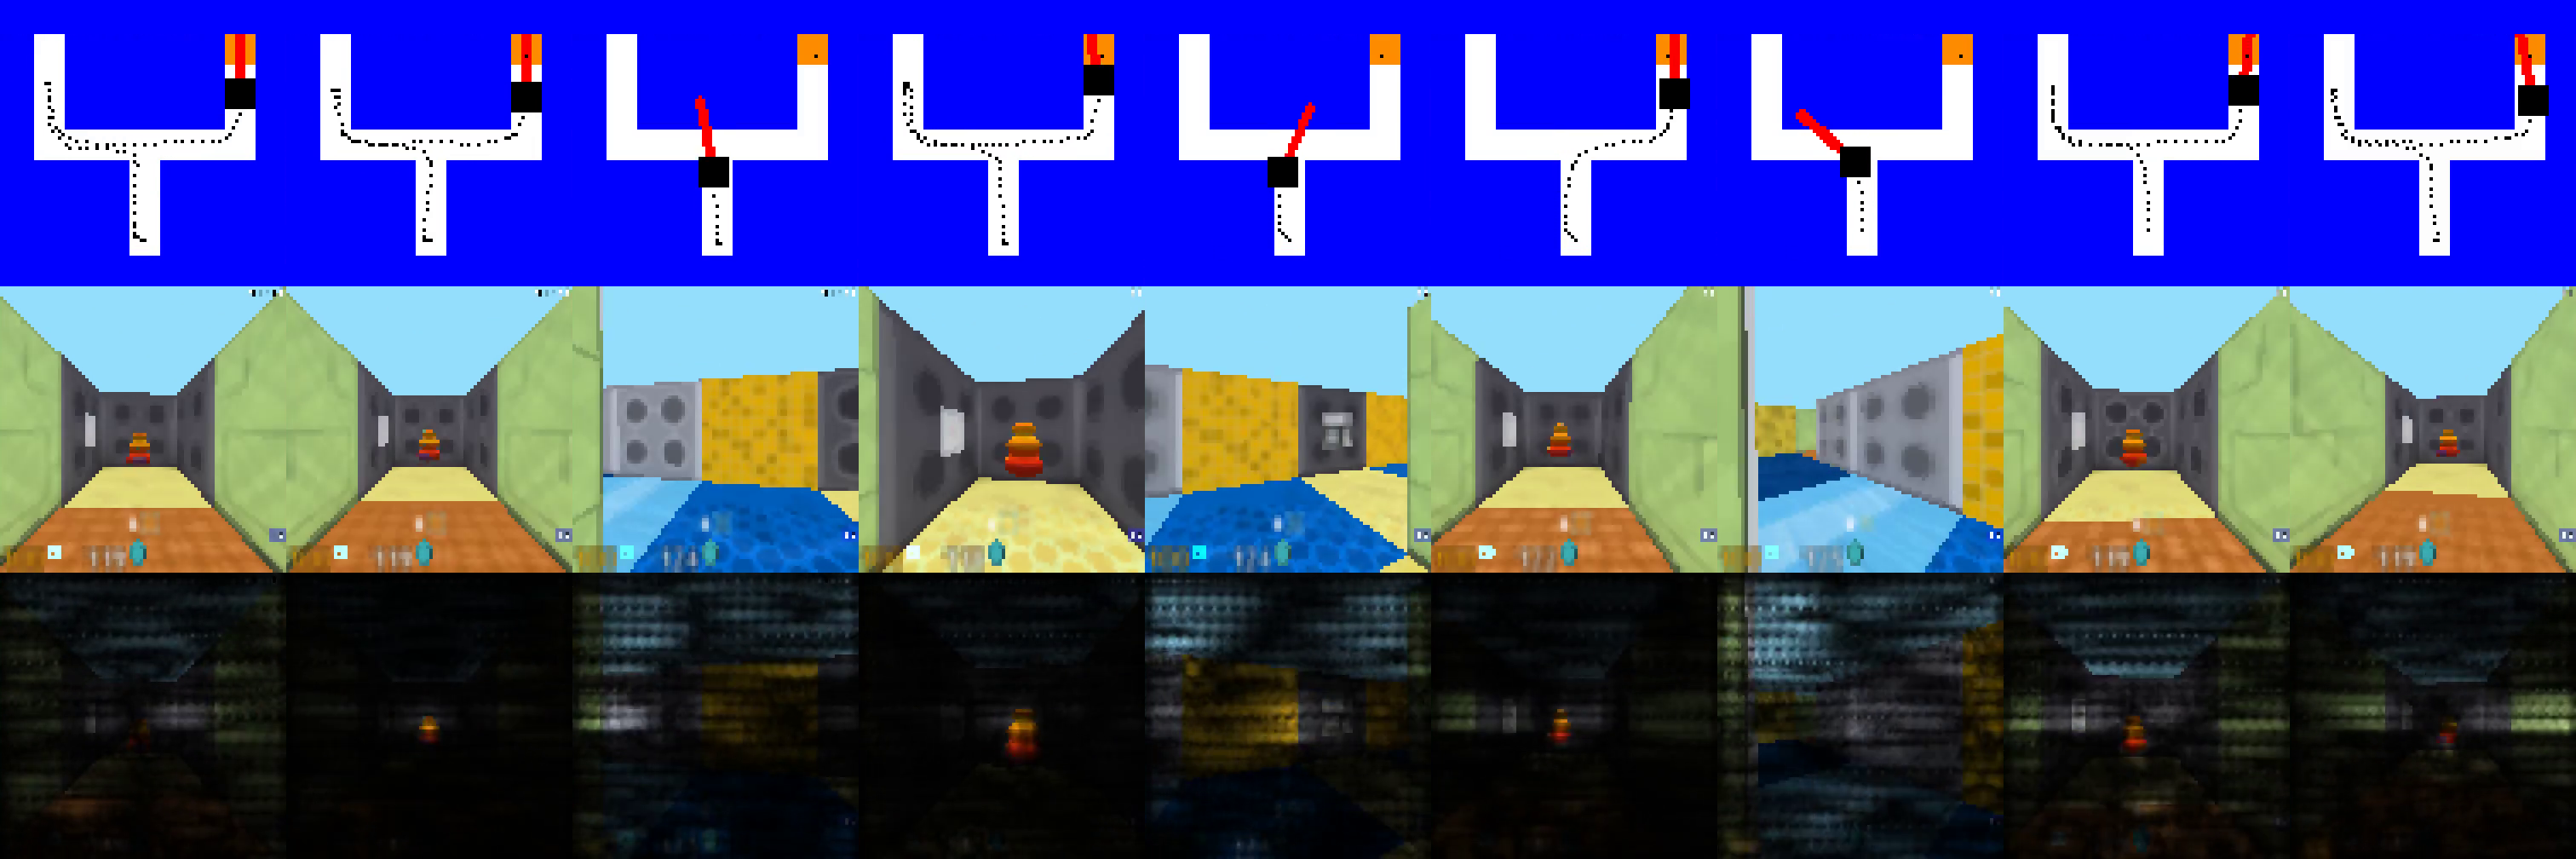
\includegraphics[width=0.98\textwidth,trim=0 672pt 0 0,clip]{./exp-results/training-1000_on_goal_map.png}%
\caption{Snapshots of path taken by the agent to reach the goal in a single episode when model trained on 1000 maps is evaluated Square, Wrench and Goal map.
  The top row shows an evaluation example on Square map, the agent takes the shortest path 6/10 times but when averaged over 100 episodes, the percentage of shortest path taken is not better than random $50.4$\% ($\pm 12.8$\%).
  Although for the example of Wrench map the agent takes the shortest path 8/10 times but when averaged over 100 episodes, the percentage of shortest path taken is reduced to $32.9$\% ($\pm 25.1$\%).
 For the Goal map, the example chosen here shows that the shortest path is only taken 1/6 times, on an average over 100 episodes, the shortest path is taken $42.6$\% ($\pm 35.1$\%) times.
}
\label{fig:planning-qualitative}
\end{figure}


\subsection{Attention Maps}
We use the normalized sum of absolute gradient of the loss with respect to the input image as a proxy for attention in the image.
The gradients are normalized for each image so that the maximum gradient is one. The attention values are then used as a soft mask on the image to create the visualization as shown in Fig~\ref{fig:attention}

We observe that the attention is uniformly distributed on the image when the agent spawns. The attention narrows down to a few pixels in the center when the agent is navigating through the corridor. It spreads to the entire image around turns and junctions. The attention also pays close attention to important objects like goal, apples and unique decals.

\begin{figure}
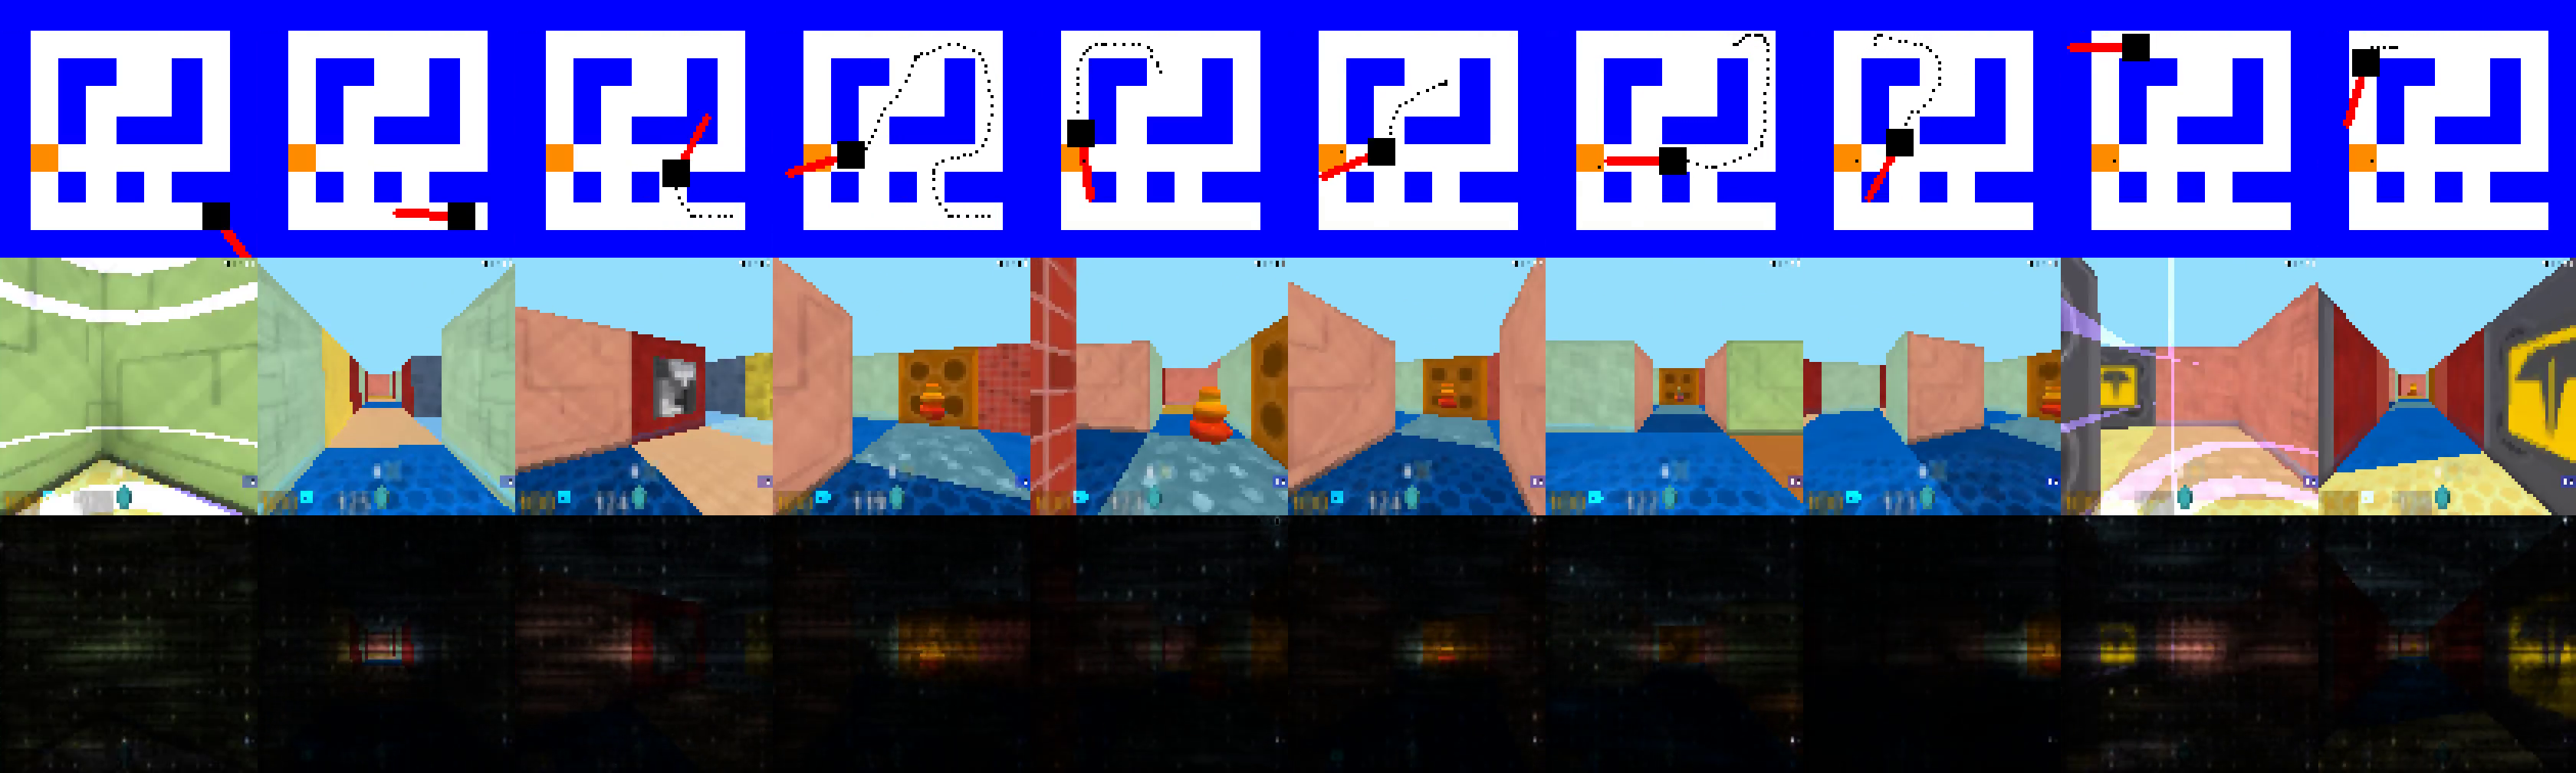
\includegraphics[width=\textwidth,trim=0 0 0 336pt,clip]{./exp-results/training-09x09-0127-on-0127.png}\vspace{1ex}\\
%
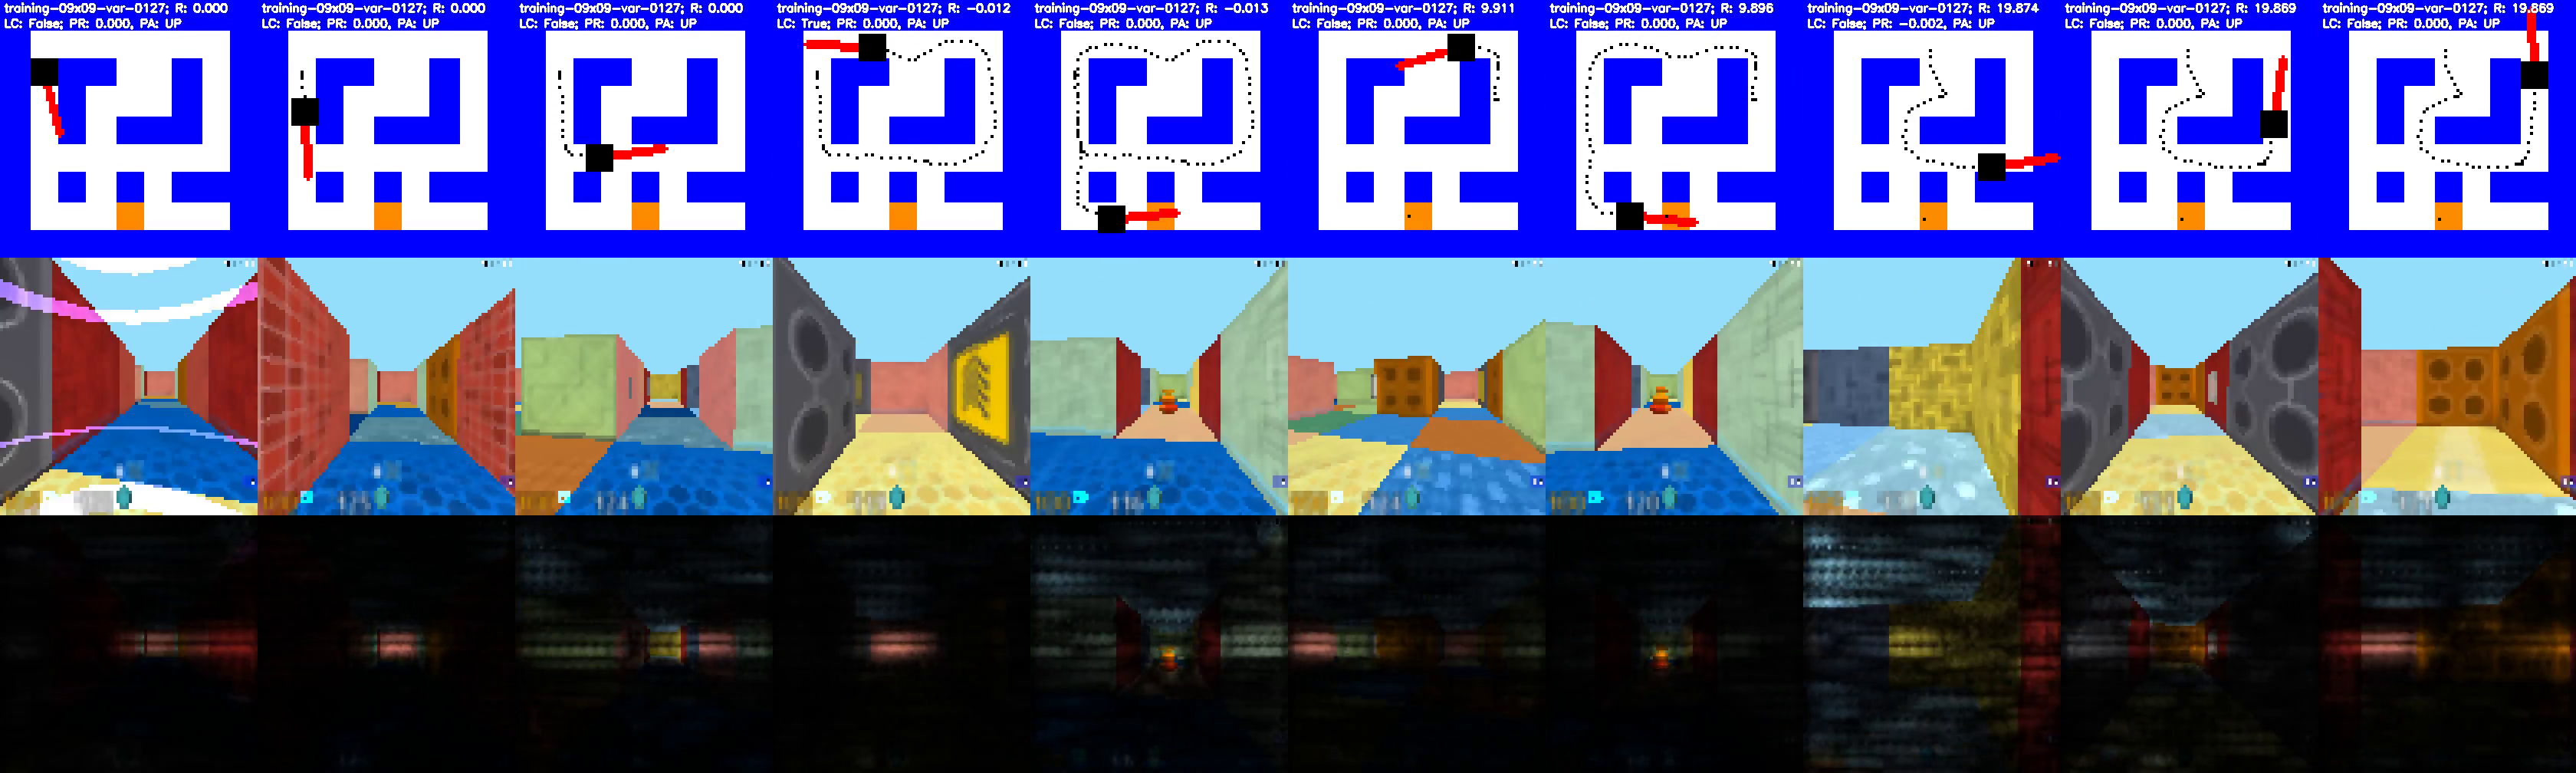
\includegraphics[width=\textwidth,trim=0 0 0 336pt,clip]{./exp-results/training-1000-on-0127.png}%
\caption{Visualizing attention for two sequences. The first two rows show the sequin when the model is trained on and evaluated on the same map. The last two rows shows the sequence for a model trained on 1000 maps and evaluated on one of the maps. We observe that the attention is uniformly distributed on the image when the agent spawns. The attention narrows down few pixels in the center when the agent is navigating through the corridor. It spreads to the entire image around turns and junctions. The attention also pays close attention to important objects like goal, apples and unique decals.}
\label{fig:attention}
\end{figure}


%Are we close to replacing the classic mapping and path-planning algorithms with DRL algorithms?
%
%As shown by the results in Fig~\ref{fig:latency-goal-reward}, the state of art DRL algorithm works well if trained and tested on the same map (static map), but performance reaches to the level of simple bug exploration like algorithms if training and testing are on different maps.





\section{Conclusion}
In this work, we comprehensively evaluate  \NavAiiiCDiDiiL{} (\cite{MiPaViICLR2017}), a DRL-based navigation algorithms, through systematic set of experiments that
are repeated over multiple randomly chosen maps.
Our experiments show that DRL-based navigation models are able to perform some degree of path-planning and mapping when trained and tested on the same map even when spawn locations and goal locations are randomized. 
However the large variation in the evaluation metrics show that how such behaviour is not consistent across episodes. 
We also train and test these methods on disjoint set of maps and show that such trained models fail to perform any form of path-planning or mapping in unseen environments.

In this work, we begin by asking: do DRL-based navigation algorithms really ``learn to navigate''?
Our results answer this question negatively. At best, we can say that DRL-based algorithms learn to navigate in the exact same environment, rather than general technique of navigation which is what classical mapping and path planning provide.
We hope that the systematic approach to the experiments in this work serve as a benchmark for future DRL-based navigation methods.



\subsubsection*{Acknowledgments}

Use unnumbered third level headings for the acknowledgments. All
acknowledgments, including those to funding agencies, go at the end of the paper.

{\small
\IfFileExists{/z/home/dhiman/wrk/group-bib/shared.bib}{
  \bibliography{/z/home/dhiman/wrk/group-bib/shared,main,main_filtered}
}{
  \bibliography{main,main_filtered}
}
\bibliographystyle{iclr2018_conference}
}


\newpage
\section*{Appendix}

\subsection*{Hyperparameters}
We use the Deepmind Lab environment to train our experiments. 
As mentioned previously, apple rewards are scattered throughout the maze and constitue a +1 reward. 
Goals constitute a +10 reward. An included wall penalty linearly penalizes the agent as it moves closer to the wall with the penalty being capped off at -.2 per frame.
Our episodes are of fixed time length ending at 40 seconds each.
The agent interacts with the environment at a rate of 30 frames per second. 
Each episode thus consists of 1200 frames of data coupled with the corresponding reward signals.
Our mazes constitute an area of $900 units \times 900 units$ though we provide the tools to generate mazes to arbitrary dimensions. 

Our A3C implementation is a modified version of OpenAIs open-sourced \emph{universe-starter-agent}. RGB images are fed in to the network of dimensions $84\times84\times3$. 16 threaded agents are used for all experiments. We use a learning rate of $10^{-4}$ along with the \emph{AdamOptimizer} to train our network. Our models train for a maximum of $10^{8}$ iterations though we end them early if maximum reward saturates. 

\subsection*{Benchmark Scores}
To motivate more comprehensive experimental evaluations of DRL-based navigation methods, we will be releasing all our trained models coupled with corresponding reward curves and videos of performance online. 
This will include completely reproducible evaluation sets wherein we display metric scores for all the trained models on the follow environments:
\begin{itemize}
    \item the original training conditions
    \item the training conditions in the absence of apples and textures
    \item the 100 unseen testing maps
    \item the planning maps i.e. the square, wrench and goal map
\end{itemize}
We hope our work can also be utilized as a stepping stone for the creation of better generalized DRL navigation methods bypassing the needless amounts of time spent engineering the infrastructure necessary for these experiments. 
All our work will be available on github after the blind-review process is over.




\end{document}
